\documentclass{anstrans}
%%%%%%%%%%%%%%%%%%%%%%%%%%%%%%%%%%%
\title{Numerical Experiments for testing Demand-Driven Deployment Algorithms}
\author{Gwendolyn Chee, Jin Whan Bae, and Kathryn D. Huff}

\institute{
Dept. of Nuclear, Plasma and Radiological Engineering, University of Illinois at Urbana-Champaign \\
gchee2@illinois.edu
}

%%%% packages and definitions (optional)
\usepackage{graphicx} % allows inclusion of graphics
\usepackage{booktabs} % nice rules (thick lines) for tables
\usepackage{microtype} % improves typography for PDF
\usepackage{xspace}
\usepackage{tabularx}
\newcommand{\SN}{S$_N$}
\renewcommand{\vec}[1]{\bm{#1}} %vector is bold italic
\newcommand{\vd}{\bm{\cdot}} % slightly bold vector dot
\newcommand{\grad}{\vec{\nabla}} % gradient
\newcommand{\ud}{\mathop{}\!\mathrm{d}} % upright derivative symbol
\newcommand{\Cyclus}{\textsc{Cyclus}\xspace}%
\newcommand{\Cycamore}{\textsc{Cycamore}\xspace}%
\newcolumntype{c}{>{\hsize=.56\hsize}X}
\newcolumntype{b}{>{\hsize=.7\hsize}X}
\newcolumntype{s}{>{\hsize=.74\hsize}X}
\newcolumntype{f}{>{\hsize=.1\hsize}X}
\newcolumntype{a}{>{\hsize=.45\hsize}X}

\begin{document}
%%%%%%%%%%%%%%%%%%%%%%%%%%%%%%%%%%%%%%%%%%%%%%%%%%%%%%%%%%%%%%%%%%%%%%%%%%%%%%%%
\section{Introduction}
For many fuel cycle simulators, it is currently up to the user to define a 
deployment scheme for each component of the fuel cycle to avoid gaps in the 
supply chain. This same goal could also be achieved by setting all the 
facility's capacities to infinity. However, this does not reflect real-world 
conditions \cite{bae_numerical_2018}. To address this gap in capability of fuel 
cycle simulators, the Demand-Driven \Cycamore Archetype project 
(NEUP-FY16-10512) is developing prediction algorithms to give \Cyclus 
demand-driven deployment capabilities. This means that \Cyclus will have the 
capability to deploy supporting fuel cycle facilities to meet front-end and 
back-end demands of the fuel cycle \cite{bae_numerical_2018}. The project is a 
collaboration between the University of Illinois Urbana-Champaign and the 
University of South Carolina. This paper will discuss the numerical experiments 
required to test the various prediction algorithms designed for the project. In 
particular, this work describes tests for the non-optimizing algorithm. 

%%%%%%%%%%%%%%%%%%%%%%%%%%%%%%%%%%%%%%%%%%%%%%%%%%%%%%%%%%%%%%%%%%%%%%%%%%%%%%%%
\section{Background: \Cyclus}
\Cyclus \cite{carlsen_cyclus_2014} is an agent-based extensible framework for modeling flow of material through user-defined nuclear fuel cycles \cite{huff_fundamental_2016}. \Cycamore \cite{carlsen_cycamore_2014} is an additional modules repository in the \Cyclus ecosystem that provides basic libraries to represent process physics of various components of the nuclear fuel cycle (ie. mining, fuel enrichment, reactor) \cite{huff_extensions_2014}. Each library is an archetype. 

\Cyclus simulations are composed of discrete time steps. Each time step is 
subdivided into phases. The time step execution phases for \Cyclus are 
illustrated in Figure \ref{fig:timeexecution}. 
Phases labeled kernel have required actions that occur and phases labeled agent are executed by individual agents. Agent refers to specific facilities within the simulation. What happens in "Tick" and "Tock" are unique to each archetype \cite{bae_numerical_2018}. 

\begin{figure}[ht] % replace 't' with 'b' to force it to be on the bottom
	\centering
	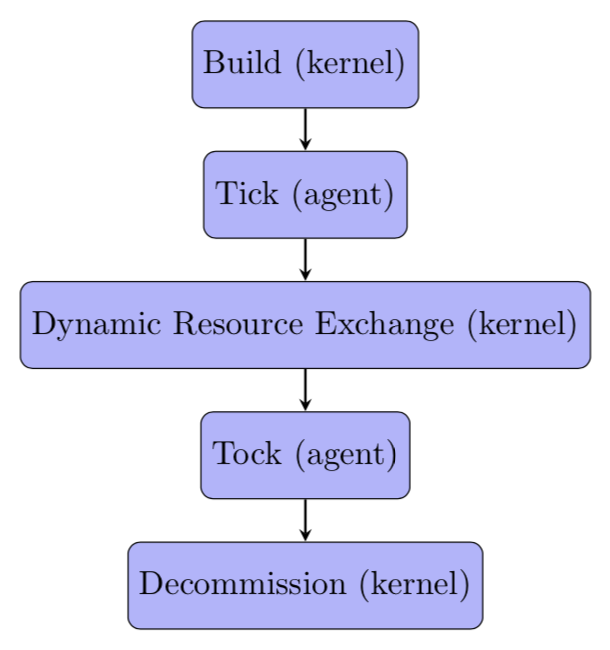
\includegraphics[width=0.29\textwidth]{timeexecution}
\caption{Each time step in \Cyclus follows the five phases in order.}
	\label{fig:timeexecution}
\end{figure}

%%%%%%%%%%%%%%%%%%%%%%%%%%%%%%%%%%%%%%%%%%%%%%%%%%%%%%%%%%%%%%%%%%%%%%%%%%%%%%%%
\section{Background: Demand-Driven Deployment Algorithms}
Nuclear fuel cycle simulation scenarios are typically best posed as constrained 
objective functions. This means that the goal of a simulation is to 
optimize an objective function with respect to constraints on certain 
variables. For nuclear fuel cycle simulations, minimizing unmet electricity 
demand or maximizing uranium utilization are typical objective functions. 
Typical constraints might limit the availability of new nuclear fuel cycle 
technology such as specific types of reprocessing. This necessitates demand 
responsive deployment capabilities to be added to fuel cycle simulation logic. 
The simulator should have the capabilities to deploy supporting fuel cycle 
facilities to enable a demand to be met. For example, for a once through fuel 
cycle with an energy growth demand of 1\% per year, the simulator should have 
the capabilities to optimally deploy supporting facilities such as a mine, 
enrichment facility and reactor to meet the demand \cite{huff_current_2017}. 

%%%%%%%%%%%%%%%%%%%%%%%%%%%%%%%%%%%%%%%%%%%%%%%%%%%%%%%%%%%%%%%%%%%%%%%%%%%%%%%%
\section{Method: Prediction Algorithms}
For this project, three prediction algorithm types are considered: non-optimizing methods, deterministic optimization and stochastic optimization. They are listed in level of effectiveness and difficulty of design. These prediction models are currently being developed by the USC team. Essentially, each algorithm will create a supply chain of reactor and supporting fuel facilities. At every time step, the demand for each fuel cycle commodity will be evaluated and the algorithm will make a prediction about future demand, resulting in the deployment or decommissioning of facilities \cite{bae_numerical_2018}. 

The non-optimizing method type is the most basic optimization algorithm. It predicts future deployment schedules solely based on historical data. In the tick phase, the difference in supply and demand for each commodity is evaluated. Based on the size of the difference and capacity of the corresponding facility, facilities will be deployed or decommissioned. Methods that are used include autoregressive moving average (ARMA) and autoregressive conditional heteroskedastic (ARCH) methods. Both ARMA and ARCH rely on an autoregressive model which means that the predicted future values of a time series depend on the previous values of that same time series \cite{scopatz_technical_2016}.

%%%%%%%%%%%%%%%%%%%%%%%%%%%%%%%%%%%%%%%%%%%%%%%%%%%%%%%%%%%%%%%%%%%%%%%%%%%%%%%%
\section{Method: Tests}
In Best Practices of Scientific computing \cite{wilson_best_2014}, Wilson et 
al. highlights the fact that similar to building experimental apparatus, 
constructing software requires careful building and validation to ensure their 
reliability. Furthermore, Wilson et al discusses that because software is 
commonly reused, it can result in a negative long term effect on the integrity 
of the group's work if a bug is not found. 

An important practice for verification and maintenance of code is to write and 
run tests. Automated tests ensure that a piece of code 
is functioning the way it is intended. The most basic test is the unit test 
which refers to the testing of a single function \cite{wilson_best_2014}. For 
the demand-driven deployment algorithms, unit tests will be written for each 
section of code to ensure all components of the code are reliable. Testing may 
not be perfect at capturing all the bugs; however, it minimizes them. 

The goal is for the demand-driven deployment algorithms to be integrated with 
the \Cyclus framework in the long term and used to optimize simulations of 
transition analyses. Therefore, if the algorithms are not well tested, they may 
have undiagnosed logic flaws or bugs. This would result in inaccuracies with 
the conclusions drawn from the transition analyses simulations and further 
compromise any experiments that use the algorithm in the future 
\cite{wilson_best_2014}. 

\subsection{Test Example} 

A simple once through fuel cycle scenario is sufficient to verify the 
non-optimizing algorithm. The scenario used has only four facilities. Figure 
\ref{fig:materialflow} depicts the material flow between the four facilities.   
In it, the bracketed values are demands calculated in the algorithm. The 
Reactor demands \textit{x} amount of fuel which translates to \textit{x} demand 
from enrichment and \textit{ax} demand from source, taking into account 
enrichment losses \cite{bae_numerical_2018}.

\begin{figure}[ht] % replace 't' with 'b' to force it to be on the bottom
	\centering
	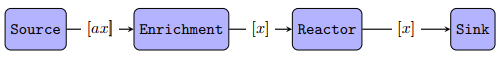
\includegraphics[width=0.48\textwidth]{materialflow}
\caption{Simple demand flow of materials.}
	\label{fig:materialflow}
\end{figure}

\begin{table}[h]
	\centering
	\begin{tabularx}{0.5\textwidth}{cff}
		\hline
		\textbf{Reactor Parameters} & \textbf{Value} & \textbf{Units} \\
		\hline
		Lifetime & 3 & Timesteps \\ 
		Power Capacity & 1000 & MWe \\
		Assembly Size & 100 & kg \\
		\# Assemblies per core & 3 & \\
		\hline
		\textbf{Enrichment Facility parameters} & \textbf{Value} & \textbf{Units} \\
		\hline 
		SWU Capacity & 2000 & SWU/timestep \\
		Enrichment SWU for 1 assembly & 528 & SWU \\
		Fuel output & 300 & kg/timestep \\
		\hline
	\end{tabularx}
	\caption {Simple once through nuclear fuel cycle scenario parameters \cite{bae_numerical_2018}}
	\label{tab:parameters}
\end{table}


A unit test is written for each function of the algorithm to test if its output matches the analytical solution for the specified test scenario \cite{bae_numerical_2018}. To ensure that the deployment and decommissioning of the facilities is appropriate, the tick phase must be working correctly. There are three main types of tests that will ensure this. The first test is that the difference between demand and supply for each commodity is below the capacity of its respective facility for all time steps. The second test is that the correct number of facilities are deployed at each time step. The third test is that the correct number of facilities are decommissioned at each time step.  

An example for each type of test described above is for the enrichment facility whose output commodity is fuel. Table \ref{tab:parameters} describes the scenario parameters that are relevant for both example tests.  

The first test example checks if the difference between enrichment facility fuel supply and reactor fuel demand is within plus-minus the output capacity of one enrichment facility for every time step. For this test, a reactor is deployed at time steps 2 and 3 and a fuel supply of 100kg is given at the initial time step. Since each reactor has 3 assemblies per core, a fuel demand of 300kg is required per reactor at the time step it is deployed. The analytical solution for this test is shown in table \ref{tab:test1}. 

\begin{table}[h]
	\centering
	\begin{tabularx}{0.5\textwidth}{assa}
		\hline
		\textbf{Timestep} & \textbf{Fuel Quantity (kg)} & \textbf{Fuel Demand (kg)} & \textbf{Difference (kg)}\\
		\hline
		1 & 100 & 0 &100\\
		2 & 400 & 300 &100\\
		3 & 400 & 300 &100\\
		\hline
	\end{tabularx}
	\caption {Analytical solution of the difference between fuel quantity and fuel demand per time step for a test scenario where a reactor is deployed at time step 2 and 3 and an initial fuel quantity of 100kg at time step 1 \cite{bae_numerical_2018}.}
	\label{tab:test1}
\end{table} 

The second test example checks if an enrichment facility is deployed when the amount of fuel available is below the fuel demand of the reactor. For this test, a reactor is deployed at time step 2. Since an enrichment facility outputs 300kg of fuel per timestep, one enrichment facility must be deployed at time step 2 to meet the fuel demand. The analytical solution for this test is shown in table \ref{tab:test2}.

\begin{table}[h]
	\centering
	\begin{tabularx}{0.5\textwidth}{ab}
		\hline
		\textbf{Timestep} & \textbf{Enrichment Facility deployment}  \\
		\hline
		1 & 0 \\
		2 & 1 \\
		3 & 0\\
		\hline
	\end{tabularx}
	\caption {Analytical solution of the number of fuel facilities deployed per time step for a test scenario where a reactor is deployed at time step 2. \cite{bae_numerical_2018}}
	\label{tab:test2}
\end{table}

\begin{table}[h]
	\centering
	\begin{tabularx}{0.5\textwidth}{ab}
		\hline
		\textbf{Timestep} & \textbf{Enrichment Facility deployment} \\
		\hline
		1 & 0 \\
		2 & 1 \\
		3 & 1 \\
		4 & 1 \\
		5 & 0 \\
		\hline
	\end{tabularx}
	\caption {Analytical solution of the number of enrichment facilities deployed per time step for a test scenario where a reactor is deployed at time step 2 and decommissioned at time step 5.}
	\label{tab:test3}
\end{table}

The third test example checks if an enrichment facility is decommissioned when the amount of fuel available is above the fuel demand of the reactor. For this test, a reactor is deployed at time step 2. Since a reactor has a lifetime of 3 timesteps, it is decommissioned at time step 5. Therefore, the enrichment facility must also be decommissioned at time step 5. The analytical solution for this test is shown in table \ref{tab:test3}.

Each of these tests will be implemented for each commodity in the supply chain. Both the Demand-Driven Deployment algorithms and tests are implemented in the Python language.   

%%%%%%%%%%%%%%%%%%%%%%%%%%%%%%%%%%%%%%%%%%%%%%%%%%%%%%%%%%%%%%%%%%%%%%%%%%%%%%%%
\section{Conclusions}
The above sections outline the types of numerical experiments that will be 
implemented to test the non-optimizing prediction algorithm for the 
Demand-Driven \Cycamore Archetype project. Implementation of these and further 
tests will ensure the reliability of the prediction algorithms.  
At present, iterative feedback between the testing team at the University of 
Illinois and the archetype development team at the University of South Carolina 
is driving targetted development of the non-optimizing agent archetype so that 
it will successfully pass the tests.

%%%%%%%%%%%%%%%%%%%%%%%%%%%%%%%%%%%%%%%%%%%%%%%%%%%%%%%%%%%%%%%%%%%%%%%%%%%%%%%%
\section{Acknowledgments}
This work is supported by U.S. Department of Energy's Nuclear Energy University Program under contract \# NEUP-FY16-10512. This is a joint project with University of South Carolina. The USC team comprising of Dr. Robert Flanagan and Dr. Anthony Scopatz is developing the prediction models. 

%%%%%%%%%%%%%%%%%%%%%%%%%%%%%%%%%%%%%%%%%%%%%%%%%%%%%%%%%%%%%%%%%%%%%%%%%%%%%%%%
\bibliographystyle{ans}
\bibliography{bibliography}
\end{document}

